\subsection{Ablauf}

Im Sequenzdiagramm \ref{abb:SequenzdiagrammSoftware} sieht man den Ablauf der ganzen Applikation, sowohl auf der Desktop 
Seite wie auch auf der Smartphone Seite. Da die Aufgabe vom Gerät völlig autonom verrichtet 
werden muss, wird nach dem Start der Android-App das Smartphone nicht mehr bedient 
und alle Interaktionen werden von der Desktop-App gesteuert. 
Wie aus dem Sequenzdiagramm zu entnehmen ist, wird auf der Android-App als erstes ein 
Foto aufgenommen, mithilfe dessen die Korberkennung erfolgt. 
Wurde das Startsignal von der Desktop-App mit übergeben, richtet sich das Gerät nach dem vom Detektor erkannten 
respektive berechneten Winkel aus und schiesst die Bälle ab. 
Danach wird das Endsignal an die Desktop-App übergeben.
Falls das Startsignal nicht übergeben wurde, wird die Korberkennung dennoch ausgeführt, 
allerdings schiesst das Gerät die Bälle nicht ab. Dies wird für das Testen benötigt, um 
zu überprüfen, ob die Korberkennung wie gewünscht funktioniert.


\begin{figure}[h!]
	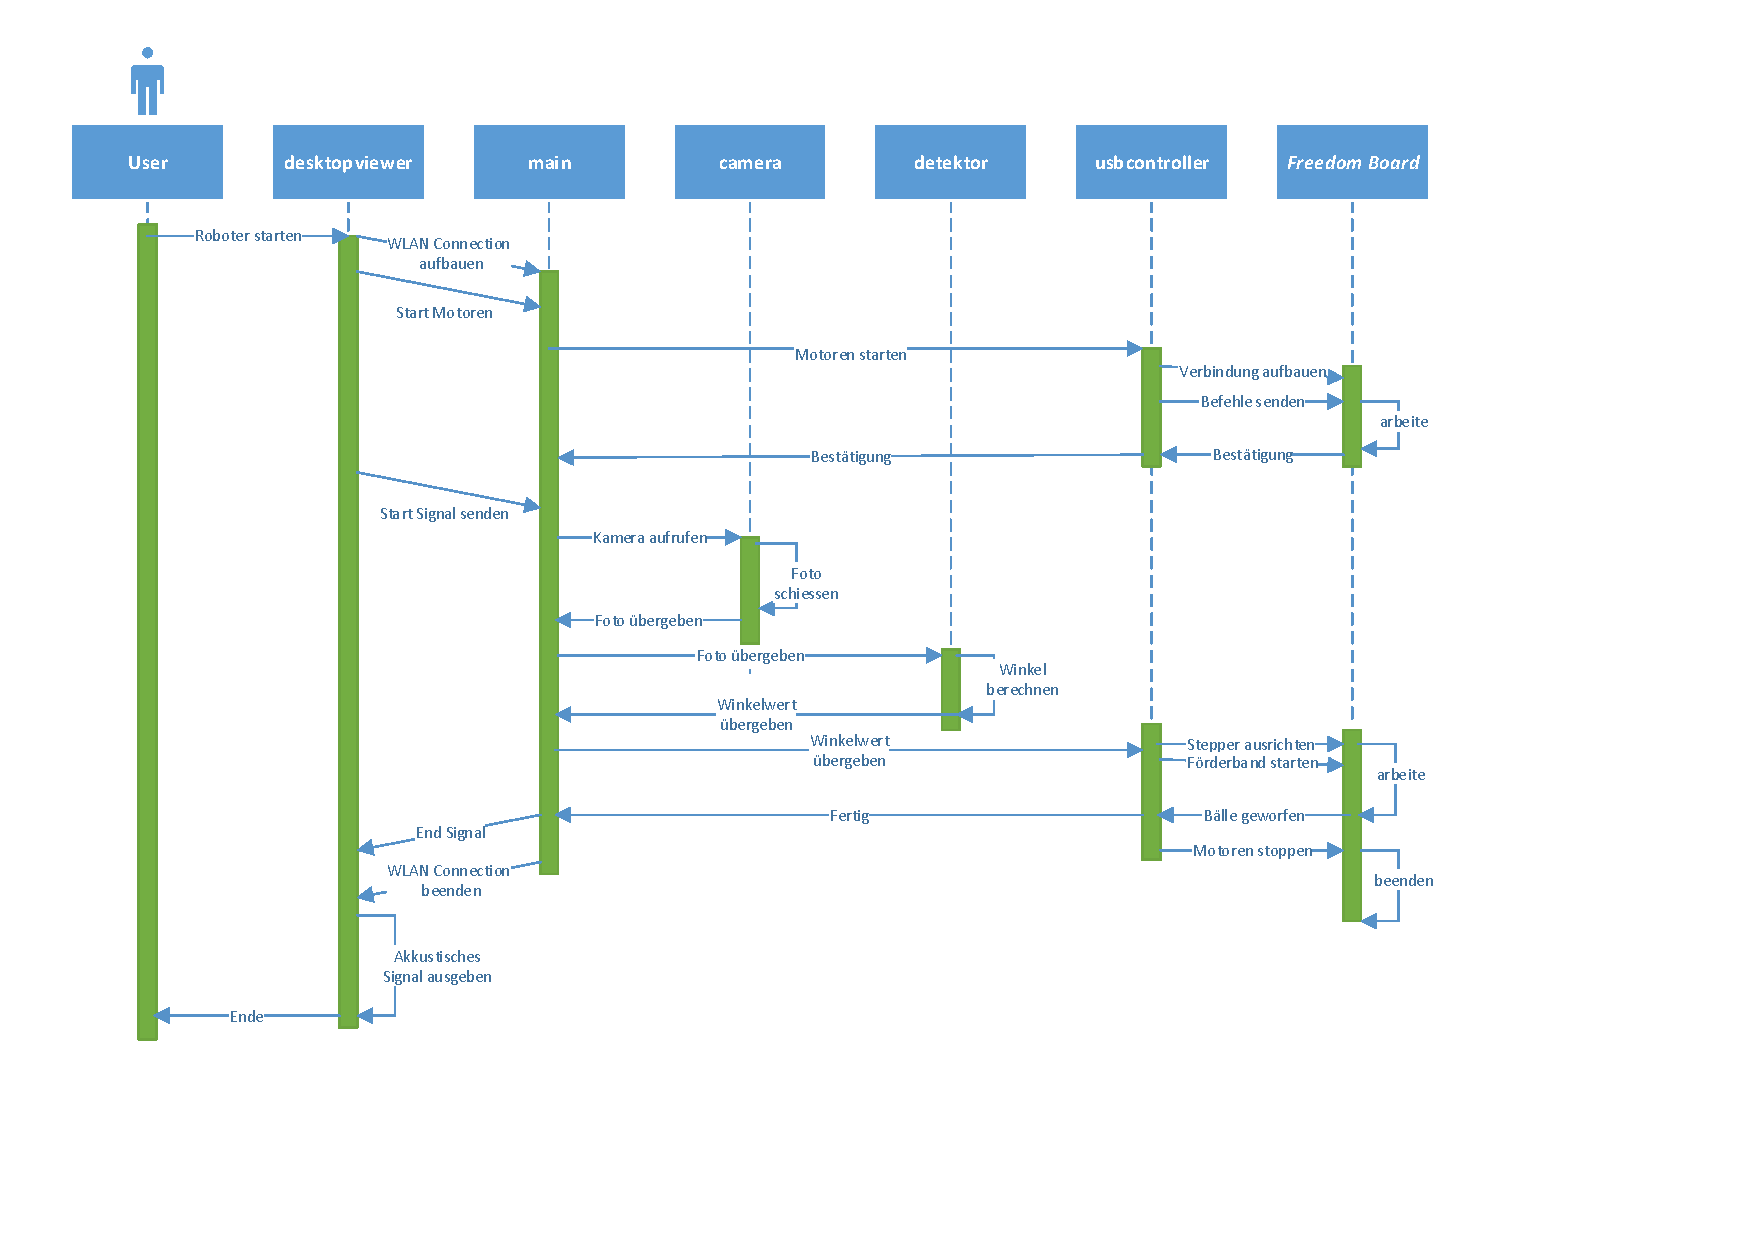
\includegraphics[width=0.95\textwidth,clip,trim=12mm 35mm 55mm 5mm]
	{Enddokumentation/Bilder/Sequenzdiagramm_PREN2_v1.pdf}
	\centering
	\caption{Sequenzdiagramm Programmablauf}
	\label{abb:SequenzdiagrammSoftware}
\end{figure}


            
